\DeclarePairedDelimiter\ceil{\lceil}{\rceil}
\DeclarePairedDelimiter\floor{\lfloor}{\rfloor}

%CHAPTER
\chapter{Implementace modulu}
Při implementaci modulu bylo třeba vybrat nejvhodnější knihovnu pro generování PDF souboru a tu následně integrovat s předem vybraným parserem. Pro snadnější integraci byly vytvořeny nové třídy.
\section{Adresářová struktura modulu}
Adresářová struktura modulu na serveru vypadá následovně:
\begin{itemize}
	\item \textbf{config} -- Adresář obsahující konfigurační soubor \textit{configuration.xml}, ve kterém jsou uložena často měněná data (rok konference, upozorňující informace aj.).  
	\item \textbf{img} -- Adresář obsahující obrázky použité v dokumentu (logo konference TSD).
	\item \textbf{lib} -- Adresář obsahující zdrojové kódy knihoven třetích stran (generátor a parser).
	\item \textbf{src} -- Adresář obsahující zdrojové kódy vytvořené autorem bakalářské práce.
	\item \textbf{orlib.php} -- Hlavní soubor modulu obsahující všechny 3 stěžejní funkce modulu.
\end{itemize}
%SECTION
\section{Implementované třídy}
Pro modul bylo vytvořeno 7 tříd rozdělených do 4 souborů, které zajišťují veškerou pomocnou funkcionalitu (vytváření formulářových prvků, konstanty aj.) při generování PDF souboru. 
%SUBSECTION
\subsection{Výčtové typy}
\textbf{Výčtový typ} (neboli \textbf{Enum}) je datový typ určený pro uložení konstant programu, kdy každé z těchto konstant je přiřazena jedna instance výčtu. Ve vytvářeném modulu byly použity 4 třídy jako výčtové typy. 
\par
Třída \textbf{Instruction} uchovává konstanty využité při generování titulku a informací během vyplňování formuláře. Tyto konstanty reprezentují celkem 4 části dokumentu (Záhlaví, Titulek dokumentu, Jméno posuzovatele a Instrukční text pro vyplňování formuláře).
\par
Třída \textbf{FormElements} slouží pouze pro rozlišení použitých objektů na základní prvky formuláře. Zde byly použity prvky \textit{Radiobutton} a \textit{Textové pole}.
\par
Ve třídě \textbf{TextareaInfo} jsou uloženy veškeré konstanty pro hodnotící parametry, které jsou reprezentovány jako \textit{Textová pole}, a pomocné funkce. Každý hodnotící parametr je zde určen třemi konstantami (jednoznačný identifikátor, název a jeho popis). Dále se tu vyskytují 2 konstanty využité při vytváření formulářového prvku pomocí HTML kódu. Tyto konstanty jsou využity i při následném zpracování dokumentu pro všechny formulářové prvky reprezentované jako textová pole. Byla zde vytvořena i funkce \textit{getNotNeededConstants} pro získání nepovinných hodnotících parametrů.
\par
Třída \textbf{RadiobuttonInfo} je téměř totožná s třídou \textbf{TextareaInfo} s tím rozdílem, že hodnotící parametry jsou reprezentovány jako \textit{Radiobutton}.
%SUBSECTION
\subsection{TCPDFElements}
Hlavním důvodem vzniku této třídy byla snaha nevytvářet formulářové prvky přímo v hlavní funkci \textit{generate\_offline\_review\_form} ale použít nově vytvořené metody. Pomocí implementovaných metod lze vytvářet textová pole, radiobuttony, textové části dokumentu a načítat vědecký příspěvek.
%SUBSECTION
\subsection{TextConversioner}
V některých případech jsou název vědeckého příspěvku nebo jméno posuzovatele příliš dlouhé, a proto narušuje vzhled výsledného dokumentu. Problém může nastat i při chybě programátora, pokud by byl instrukční text příliš rozsáhlý. Proto byla vytvořena třída \textbf{TextConversioner}, která má za úkol nejdříve zkontrolovat předaný text a porovnat ho se stanovenými konstantami určujícími maximální délku textu. Pokud je rozsah textu delší než stanovená délka, tak se následně vypočte potřebný font pro vykreslení celého textu pomocí vzorce \eqref{eq:font_size}, která se porovnává se stanovenými konstantami určujícími minimální font. 
\begin{equation}
newFontSize = \floor*{\frac{maxTextLength}{textLength} \cdot fontSize} \label{eq:font_size}
\end{equation}

Pokud je vypočtený font je menší než předem stanovený minimální font, je text zkrácen na velikost vypočtenou pomocí vzorce  \eqref{eq:text_length} a doplněn třemi tečkami na jeho konci. 

\begin{equation}
newLength = \floor*{\frac{oldFontSize}{minFontSize} \cdot textLength} \label{eq:text_length}
\end{equation}
%SUBSECTION
\subsection{ConfigurationData}
Třída načítá veškerý obsah konfiguračního souboru, který následně ukládá do svých proměnných. Data uložená v konfiguračním souboru slouží pro nastavení textu vodoznaku a jako informační text pro uživatele.
%SECTION
\section{Generátor}
Generátor by měl být při vytváření PDF dokumentu rychlý, vykreslit co nejpřesněji prvky webového formuláře do vygenerovaného dokumentu a nebýt implementačně náročný.
%SUBSECTION
\subsection{TCPDF x mPDF}
Při analyzování dostupných PHP knihoven pro generování PDF souborů byly nalezeny 2 vyhovující knihovny, které mohou potencionálně splňovat potřebnou funkcionalitu, bohužel pouze jedna může být použita do vyvíjeného modulu. Po vytvoření jednoduchého souboru obsahujícího základní formulářové prvky bylo rozhodnuto, že knihovna \textbf{mPDF} bude použita pro generování PDF souborů. Důvody této volby jsou popsány níže.
\par
Za jeden z důležitých faktorů lze označit skoro kompletní podporu \textit{CSS3} (Cascading Style Sheets 3) u \textbf{mPDF}, díky čemuž lze dosáhnout perfektního nastavení stylů pro jednotlivé objekty v dokumentu. Naproti tomu \textbf{TCPDF} nepodporuje značné množství CSS parametrů, například parametr určující šířku vnějšího okraje prvku, a pro dosažení obdobného výsledku je zapotřebí značné množství jiných parametrů definující styl prvku.
\par
Důležitým faktorem při vytváření PDF dokumentu je rychlost generování a paměťová náročnost. V tabulce \ref{tab:table_generators} lze vidět porovnání knihoven pro 2  PDF soubory, kdy první PDF obsahovalo hlavně CSS styly, zatímco v dlouhém PDF byla vytvořena tabulka s více jak tisíci záznamy.
\begin{table}[h!]
\centering
\begin{tabular}{|l|l|l|l|l|} 
\hline
\textbf{Název} & \multicolumn{2}{l|}{\textbf{Komplexní PDF}} & \multicolumn{2}{l|}{\textbf{Dlouhé PDF}}  \\ 
\hline
               & \textbf{Paměť [MB]} & \textbf{Čas [ms]}     & \textbf{Paměť [MB]} & \textbf{Čas [ms]}   \\ 
\hline
TCPDF (v6.2.13)          & 74                  & 35944                 & 2,3                 & 96350               \\ 
\hline
mPDF   (v7.1.6)           & 14                  & 11316                 & 22,5                & 4120                \\
\hline
\end{tabular}
\caption{Tabulka časové náročnosti a využité paměti při generování}
\label{tab:table_generators}
\end{table}
\par
Posledním a zároveň rozhodujícím faktorem je psaní PHP kódu pro vykreslování obsahu, kdy při vytváření kódu u \textbf{mPDF} se využívá minimum funkcí pro nastavení parametrů PDF souboru jako jsou například metadata, zatímco veškeré zobrazené elementy a text jsou psány v HTML stylu, se kterým se snadno pracuje. V mPDF lze snadno měnit parametry jednotlivých elementů, což bude oceněno hlavně u parseru. U \textbf{TCPDF} se zobrazovaný obsah vkládá pomocí předem vytvořených funkcí, přičemž tyto funkce mohou obsahovat mnoho parametrů, které si uživatel obtížně zapamatuje a vždy bude potřebovat patřičnou dokumentaci pro správné použití, což bude zabírat mnoho času při vyvíjení nových modulů.
\par
Na závěr porovnání lze říci, že ve většině případů je vhodné využít pro generování PDF souborů knihovnu \textbf{mPDF}. Pokud by bylo nutné vytvořit dokument například ve stylu knihy s nulovým využitím CSS stylů a potřebou kvalitního vysázení textu, pak je lepší použít knihovnu \textbf{TCPDF}. 

%SUBSECTION
\subsection{Popis vytvoření dokumentu}
Na samotném začátku generování jsou definovány veškeré proměnné vytvořených tříd. U proměnné, která reprezentuje třídu \textbf{ConfigurationData}, proběhne i načtení dat z konfiguračního xml souboru. Dále jsou vytvořeny proměnné reprezentující název vybraného dokumentu a informace o nahrání vyplněného dokumentu do webového portálu konference TSD. Před samotným začátkem generování je do modulu importováno CSS nastavení pro vzhled celého dokumentu.
\par
V první části generování probíhá přiřazení CSS stylů k jednotlivým HTML položkám (použité fonty, velikosti fontů aj.), které je doprovázeno vytvořením záhlaví. Pro celý dokument je použit font \textit{Helvetica}, pouze vyjímečně je zařazen font \textit{Times New Roman}, například pro titulek dokumentu a text se stylem \textit{Bold}. Do záhlaví byl vložen identifikátor hodnotícího příspěvku doplněn o název hodnoceného vědeckého příspěvku, který je případně zkrácen na určitou délku, pokud nesplňuje limity nastavené ve třídě \textbf{TextConversioner}, a logo konference TSD. 
\par
V druhé části generování proběhlo vložení vodoznaku do celého dokumentu, uložení jednoznačného identifikátoru jak hodnoceného vědeckého příspěvku, tak i hodnotícího příspěvku do příslušných metadat dokumentu. Na první stránce dokumentu je vykreslen titulek s identifikátorem hodnoceného vědeckého příspěvku, název hodnoceného vědeckého příspěvku (případně zkrácen stejně jako u záhlaví), jméno posuzovatele a doprovodný text při vyplňování hodnotícího formuláře. Pod tímto textem je vykreslena první část hodnotícího formuláře, která obsahuje 8 skupin radio buttonů a 1 textové pole.
\par
Ve třetí a poslední části probíhá vykreslování zbylých čtyř textových polí, kde 2 poslední z nich jsou nepovinná. Za hodnotícím formulářem je vložen kompletně celý hodnocený vědecký příspěvek, jehož obsah se uloží do modulu a následně stránku po stránce je přidáván do generovaného PDF dokumentu.
%SUBSECTION
\subsection{Nedostatky v mPDF}
Při vytváření dokumentu byly nalezeny 2 chyby znemožňující úplné vykreslení celého dokumentu. Níže jsou tyto chyby popsány i s návrhem jejich řešením.
\par
První chyba byla zjištěna na úplném začátku implementace generátoru, kdy při vkládání textových polí do formuláře se po přeložení kódu nevytvořil žádný dokument. Při zkoumání zdrojového kódu knihovny a vytvoření testovacích dokumentů bylo zjištěno, že knihovna neumožňuje použít textové pole, pokud se při jeho vytvoření nezadá vkládaný text. Proto bylo nutné upravit kód knihovny, konkrétně ve vykreslování textového pole. Aby bylo možné takto upravovat zdrojový kód knihovny, tak nesmí být knihovna pod licencí a naopak musí  být alespoň pod licencí dovolující úpravy, například \textit{GNU General Public License} verze 2, pod kterou je licencována i mPDF. Pro vyřešení tohoto problému byl přidán mechanismus, který při vytváření prázdného textového pole přidá znak \uv{\textbf{a}} (viz \ref{lst:elements_a}) a posléze je v knihovně při vykreslování textového pole tento znak odstraněn, což nemá vliv na jakýkoliv jiný znak či slova než zmiňovaný znak \uv{\textbf{a}}, viz \ref{lst:mpdf_a}.
\begin{lstlisting}[caption = {Dočasné přiřazení znaku \uv{\textbf{a}} do textového pole (HTMLElements.php)}, label = {lst:elements_a}, captionpos=b]
if($textarea_text == '') $textarea_text = 'a';
\end{lstlisting}
\begin{lstlisting}[caption = {Odstranění znaku \uv{\textbf{a}} z textového pole (Mpdf.php)}, label = {lst:mpdf_a}, captionpos=b]
if (isset($objattr['text']) && $objattr['text'] != 'a') {
	$texto = $objattr['text'];
}
else $texto = '';
\end{lstlisting}
\par
Druhá chyba byla nalezen při testování zkracování délky textu titulku, pokud překročí nastavenou mez. V aktuální verzi PHP se vyskytuje problém, který zneplatňuje některé UTF-8 znaky. Pokud je například vytvořen nový uživatel se jménem obsahující například znak \uv{\textbf{ř}}, pak se tento znak nepřevede správně a bude vykreslen jako neznámý znak. Bohužel generování dokumentu neprobíhalo správně, protože knihovna mPDF tyto znaky nerozpoznala, a proto výsledek vždy skončil chybou. Ze všech vyzkoušených možností, jako například změna kódování textu titulku nebo nahrazení neplatných znaků prázdnými, fungovala pouze jedna, a to nastavení atributu \textbf{ignore\_invalid\_utf8} na \textit{true} u proměnné třídy \textit{Mpdf} (viz \ref{lst:ignore_invalid_utf8}).
\begin{lstlisting}[caption = {Nastavení atributu \textbf{ignore\_invalid\_utf8} (orlib.php)}, label = {lst:ignore_invalid_utf8}, captionpos=b]
$mpdf->ignore_invalid_utf8 = true;
\end{lstlisting}

%SECTION
\section{Parser}
Z analýzy knihoven pro zpracování PDF dokumentů splnil nutné požadavky pouze \textbf{PDF Parser}.Při implementování parseru bylo zjištěno, že jednotlivé PDF prohlížeče při uložení PDF dokumentu využívají jiné komprimační metody, pracující s novějšími verzemi PDF pro určité funkce a některé prohlížeče ukládají objekty v dokumentu na více místech (duplikace, jednou komprimovaně, jednou nekomprimovaně).

%SUBSECTION
\subsection{Popis zpracování dokumentu}
Zpracování dokumentu začíná ihned po jeho nahrání do webového portálu konferenčního systému, kdy se veškerá raw data předají do PDF Parseru. Před samotnou extrakcí dat jsou pomocí TCPDF parseru, který je součástí PDF Parseru, raw data rozdělena na objekty pomocí \textit{traileru} a \textit{xref tabulky}. Následně jsou objekty dekódovány a předány PDF Parseru, který s nimi dále pracuje. Ihned po předání jsou tyto objekty dále zpracovávány podle specifických znaků, které se vyskytují v datech, například v objektu \textit{Slovník} se na samém začátku vyskytují znaky \uv{<<}. Zároveň se kontroluje název objektu, podle kterého lze zjistit o jaký typ formulářového prvku se jedná. Každý prvek formuláře má přiřazen jednoznačný název. Jako příklad lze uvést textové pole, které má při generování přiřazen název \uv{textareaID}, kde ID je jednoznačný identifikátor textového pole, který je deklarován ve výčtovém typu \textbf{TextareaInfo}. Pokud je název totožný se specifickým názvem jakéhokoliv formulářového prvku, který je v modulu naimplementován, tak je potom ihned uložen do struktury, která je po dokončení parsování poslána do modulu. 
\par
Po zpracování celého dokumentu jsou požadované objekty roztříděny na základě jejich jednoznačných identifikátorů (čísla na konci slovního identifikátoru, například \uv{\textit{textarea\textbf{0}}}, kde \textbf{0} popisuje v modulu hodnotící parametr \textit{Originality}). Před uložením hodnot jsou tyto parametry testovány, jestli jsou náležitě vyplněny, což platí pouze pro povinné položky. Zpracování probíhá pro každý základní prvek formuláře samostatně ideálně pomocí cyklu a switche. V případě, že všechna povinná pole jsou vyplněna a neproběhla žádná chyba ve zpracování, jsou všechny hodnotící parametry uloženy do databáze webového portálu konference TSD.
\par
Při nahrávání dokumentu může dojít k několika chybám, kterých se posuzovatel může dopustit, a proto jsou náležitě ošetřeny.
\begin{itemize}
	\item \textbf{Neplatné PDF} -- Posuzovatel při nahrávání dokumentu zvolí nevalidní PDF dokument (nevygenerovaný webovým portálem).
	\item \textbf{Neplatný identifikátor hodnotícího příspěvku} -- Posuzovatel může při nahrávání zvolit hodnotící PDF dokument patřící k jinému hodnocení vědeckého příspěvku (posuzovaní identifikátoru hodnotícího příspěvku a vědeckého příspěvku).
	\item \textbf{Nevyplněné požadované parametry} -- Nahrávaný PDF dokument obsahuje nevyplněné povinné hodnotící parametry. Tyto parametry jsou vypsány v chybovém hlášení zobrazeném po pokusu nahrát PDF dokument do webového portálu.
	\item \textbf{Databázové chyby} -- Při ukládání dat do databáze webového portálu může dojít k neočekávané chybě, která zapříčiní nesprávné uložení dat. 
	\item \textbf{Uzavřené hodnocení příspěvku} -- Posuzovatel nahraje hodnotící PDF dokument do webového portálu, zatímco hodnocení vědeckého příspěvku je uzavřeno administrátorem webového portálu.
\end{itemize}

%SUBSECTION
\subsection{Extrakce formulářových prvků z předpřipravených dat}
%VLOŽIT SEM MŮJ VÝKONNÝ KÓD V PDF PARSERU, POPSAT JEHO STRUKTURU A MENŠÍ INFO
TCPDF parser částečně extrahuje veškeré PDF objekty do svých struktur, které jsou následně poslány do PDF Parseru, který je pomocí svých funkcí a tříd rozdělí na základě datového typu vyplněného obsahu, jako je například prostý text, datum nebo číselná hodnota. Příklad struktury jednotlivých objektů lze vidět na obrázku \ref{fig:parsing_object}. Tento obrázek ukazuje pouze část struktury, která je mnohem rozsáhlejší a každým krokem parseru se rozkládá na menší díly.

\begin{figure}[h!]
\centering
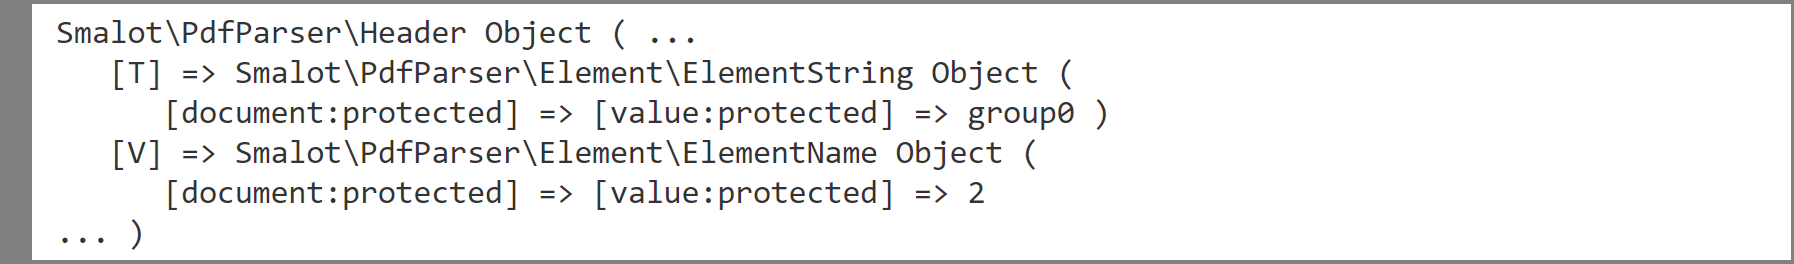
\includegraphics[width=15cm]{img/parsing_object}
\caption{Část dat PDF objektu}
\label{fig:parsing_object}
\end{figure}
\par
Pro extrahování dat a zjištění typu formulářového prvku byla vyvinuta metoda \textit{extractElement} viz \ref{lst:extraction_function}.
\begin{lstlisting}[caption = {Funkční kód pro uložení formulářových prvků z PDF objektů}, label = {lst:extraction_function}, captionpos=b]
protected function extractElement($header) {
   $elementKey = $header->getElements()['T'];                                                      
   if ($elementKey != null) {
      if (strpos($elementKey->getContent(), 'group') !== false) $type = 'groups';
      else if (strpos($elementKey->getContent(), 'textarea') !== false) $type = 'textareas';
                       
      if ($type != null) {
         $key = $elementKey->getContent();
         $elementValue = $header->getElements()['V'];
         if ($elementValue != null) {
            $value = $elementValue->getContent();
         }    
      }
   }
}
\end{lstlisting}
Kód na samém začátku kontroluje, zda je aktuálně zpracovávaný objekt pojmenován. To je zjištěno na základě indexu \uv{\textbf{T}} (T - Type) v poli elementů. Pokud název existuje, zjišťuje se zda se jedná o textové pole nebo skupinu radio buttonů. Za předpokladu, že typ objektu je validní, je kontrolována hodnota na základě indexu \uv{\textbf{V}} (V - Value) v poli elementů. Jakmile objekt obsahuje hodnotu, jsou do parseru vráceny všechny tři hodnoty (název formulářového prvku, typ formulářového prvku a jeho hodnota), které parser uloží do pole všech extrahovaných prvků.

%SECTION
\section{Výsledný vzhled PDF formuláře}
Výsledný vzhled PDF formuláře lze vidět na přiloženém PDF souboru níže. Před formulářem je instrukčí text vysvětlující hodnocení prvních 8 hodnotících parametrů. Protože se v některých případech stávalo, že uživatelé otevřeli tento dokument ve webovém prohlížeči, který umožňuje pouze otvírat soubory, nikoliv ukládat, byl zde přidán pokyn využívat PDF prohlížeč Adobe Acrobat, ale je možné využívat i jiné prohlížeče, které podporují vyplňování formulářů. Na konec formuláře byl přidán informační text popisující, jak má uživatel vyplněný formulář nahrát do webového portálu konference TSD. Obsah vědeckého příspěvku zde nebyl přidán z důvodu nevhodnosti prezentování práce někoho jiného.
\newpage
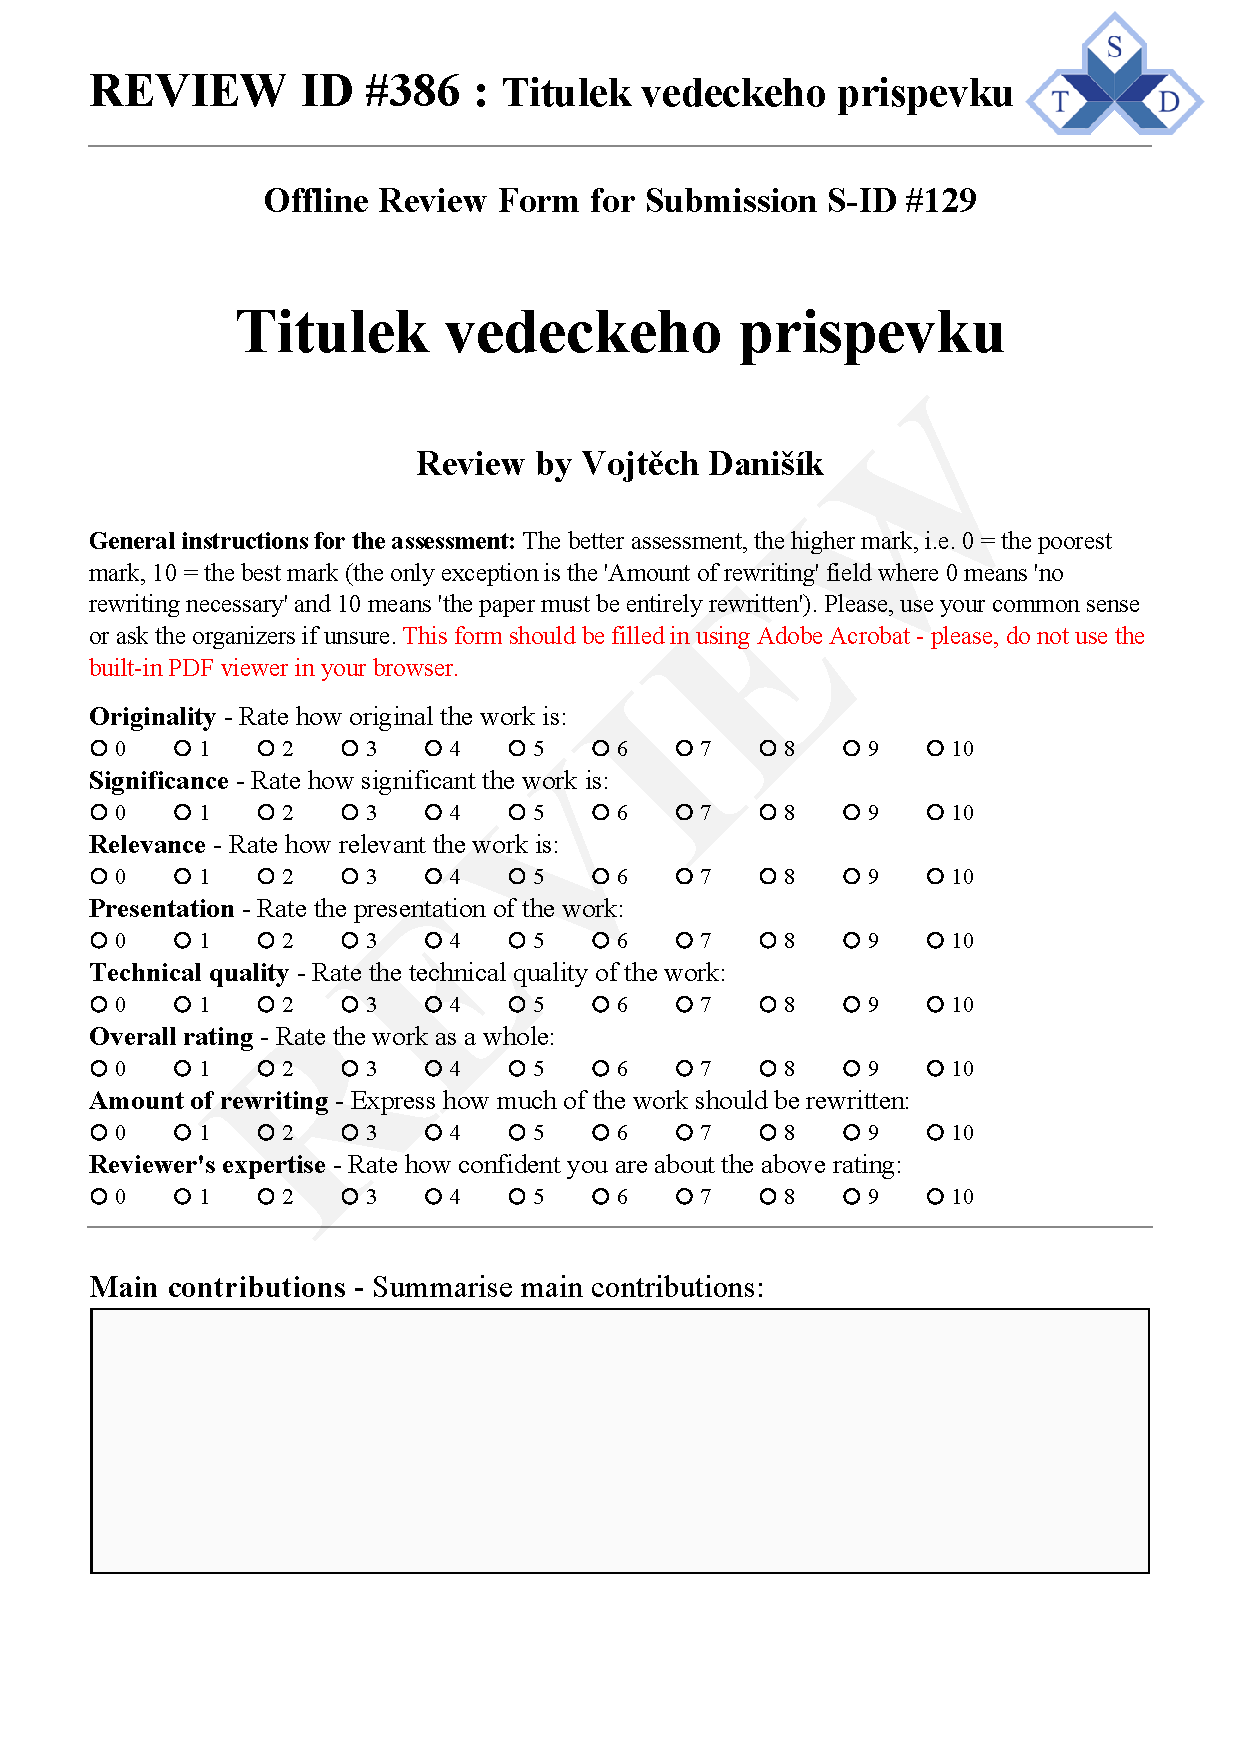
\includepdf[pages=1,pagecommand={},width=1.3\textwidth]{pdf/vysledny_vzhled.pdf}
\newpage
\includepdf[pages=2,pagecommand={},width=1.3\textwidth]{pdf/vysledny_vzhled.pdf}

%SECTION
\section{Technické požadavky}
Technické požadavky pro bezproblémové fungování TCPDI a PDF Parser jsou:
\begin{itemize} 
	\item \textbf{PHP verze} --TCPDI  momentálně funguje na všech verzích PHP, zatímco u PDF Parseru je potřeba minimální verze 5.3. Proto je nutné mít na serveru PHP verzi alespoň 5.3.0.
	\item \textbf{Podpůrné knihovny} -- Při kompresi stránek PDF souborů pomocí knihovny TCPDI je potřeba mít na serveru povoleno rozšíření \textbf{php-zlib}.
\end{itemize}
